\newpage
\section{Wyniki symulacji}
\subsection{Wyznaczenie granicznej wartości $\lambda$, dla której nie stracono żadnego użytkownika}
Aby wyznaczyć wartość graniczną, uruchomiono symulację dla wartości $\lambda$ z zakresu $<10; 50>$ użytkowników na sekundę, z krokiem 5. Każda próbka została uśredniona z 10 iteracji. W trakcie symulacji logika odpowiadająca za usypianie stacji była wyłączona. Wizualizację wyników, zrealizowaną skryptem wspomnianym w sekcji \ref{python_scripts}, przedstawiono na rysunku \ref{dropped_users_lambda}. Ostatnią wyznaczoną wartością $\lambda$, dla której nie stracono żadnego użytkownika, to 30 użytkowników na sekundę.
\begin{figure}[h]
\center
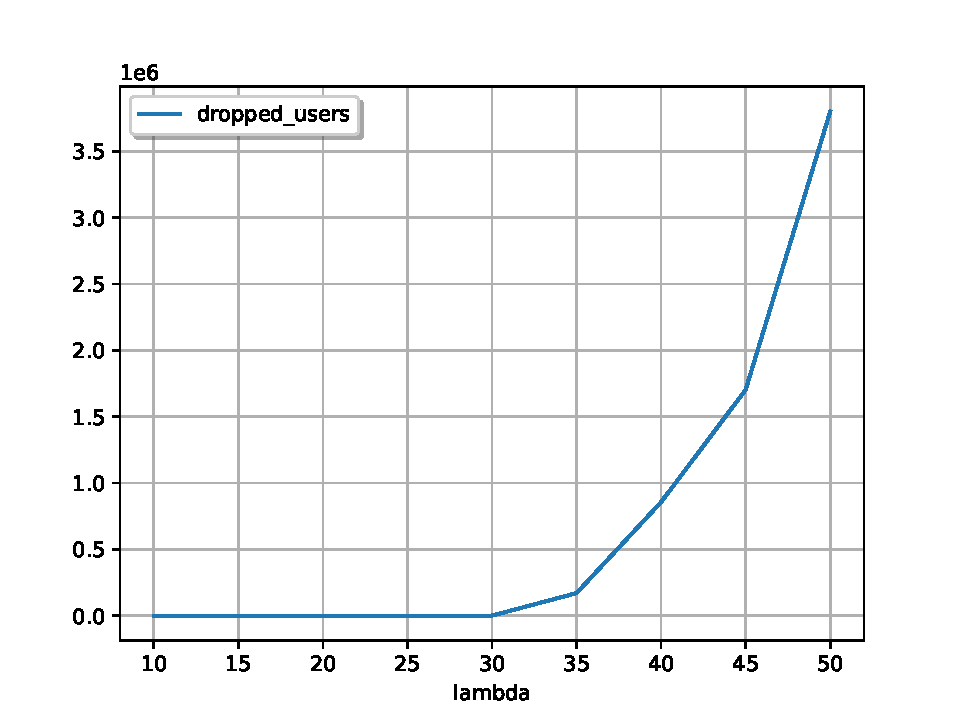
\includegraphics[scale=0.65]{img/dropped_users_lambda.pdf} 
\caption{Wykres liczby traconych użytkowników w funkcji wartości parametru $\lambda$}
\label{dropped_users_lambda}
\end{figure}

\subsection{Wyznaczenie granicznej wartości progu L, dla której straty użytkowników są poniżej 5\%}\label{drop_rate_5_section}
Aby wyznaczyć wartość graniczną, uruchomiono symulację dla wartości progu L z zakresu $<5; 40>\%$, z krokiem 5. Każda próbka została uśredniona z 10 iteracji. W trakcie symulacji parametr $\lambda$ wynosił 35. Wynik symulacji przedstawiono na rysunku \ref{dropped_users_iter_l}. Z wyników symulacji wynika, że ilość traconych użytkowników w systemie nie zależy od wartości progu L. Eksperyment powtórzono dla wartości $\lambda$ 40 oraz 50, których wyniki przedstawiono na rysunkach \ref{dropped_users_iter_l2} i \ref{dropped_users_iter_l3}. W każdym przypadku różnice pomiędzy uzyskanymi wynikami są pomijalnie małe. Wynika to najprawdopodobniej z zastosowanego algorytmu usypiania i wybudzania stacji bazowych. Analizując wykres zużycia zasobów stacji w czasie, przedstawionego na rysunku \ref{usage_over_time}, można zauważyć, że badana wartość utrzymuje się na w przybliżeniu stałym poziomie zależnym od współczynnika $\lambda$. Aby wygenerować straty użytkowników przekraczające 5\%, parametr $\lambda$ powinien być duży, na przykład z zakresu $<50;70>$ użytkowników na sekundę, aby zapełnić bloki zasobów we wszystkich stacjach. Zakres ten został wyznaczony osobnymi symulacjami, z wyłączoną logiką odpowiadająca za usypianie i wybudzanie stacji. Duża wartość parametru $\lambda$ jest także wymagana aby w systemie pojawiła się wystarczająca liczba użytkowników, aby przepełnić aktywne stacje, zanim zostanie wybudzona stacja uśpiona. Natomiast aby próg L, wskazujący poniżej jakiej wartości stacja bazowa może przejść w stan uśpienia, miał wpływ na przebieg symulacji, wartość parametru $\lambda$ musi być niska, aby zużycie bloków zasobów stacji spadło poniżej progu L. Jest to sprzeczne z postawionymi wcześniej założeniami i dlatego taka sytuacja nie zachodzi w systemie, dla podanych w treści zadania parametrów. Dlatego do dalszej części tego zadania, opisanego w sekcji \ref{get_params_section} przyjęto następujące parametry symulacji:
\begin{itemize}
\item Lambda = 43 użytkowników na sekundę
\item L = 20\%
\end{itemize}

\begin{figure}[h!]
\center
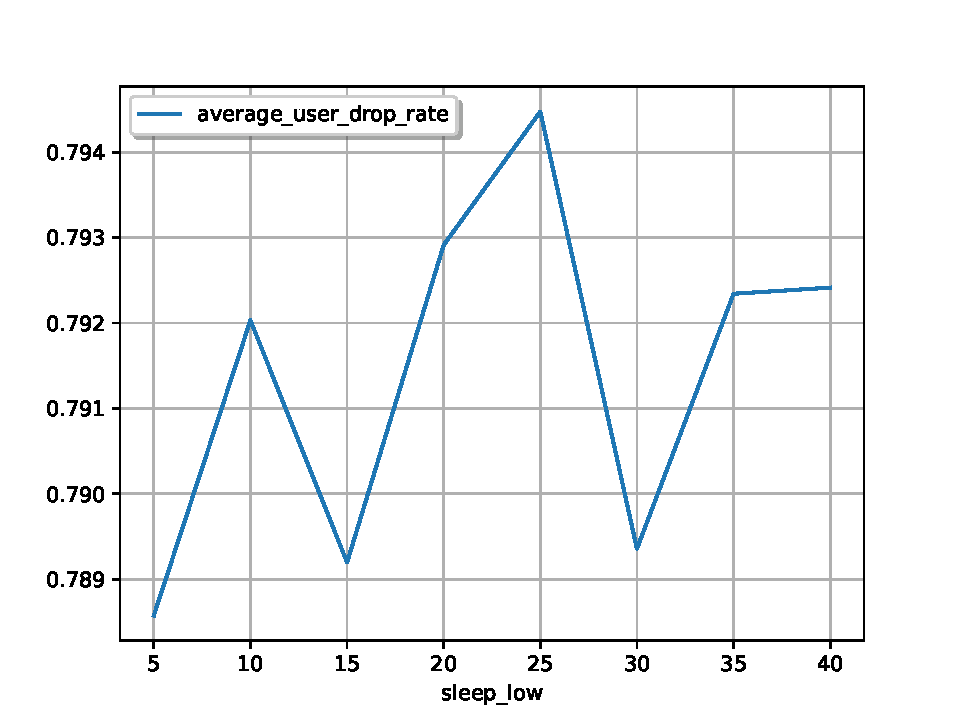
\includegraphics[scale=0.65]{img/drop_rate_lambda_35.pdf} 
\caption{Wykres procentu traconych użytkowników w funkcji wartości parametru L. W trakcie symulacji parametr $\lambda$ wynosił 35.}
\label{dropped_users_iter_l}
\end{figure}
\begin{figure}[h!]
\center
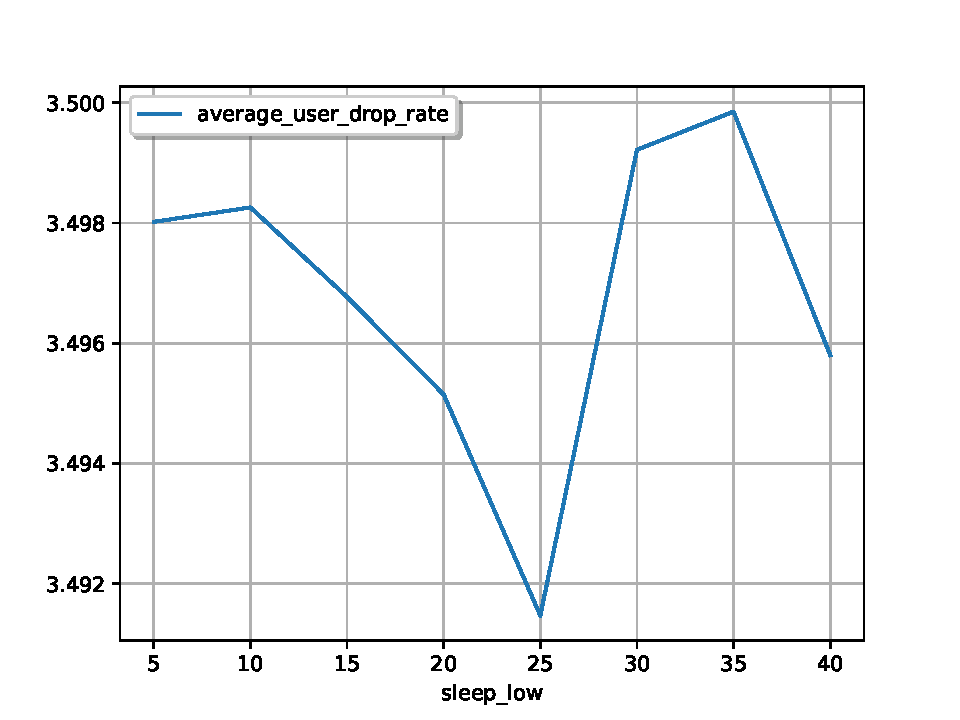
\includegraphics[scale=0.65]{img/drop_rate_lambda_40.pdf} 
\caption{Wykres procentu traconych użytkowników w funkcji wartości parametru L. W trakcie symulacji parametr $\lambda$ wynosił 40.}
\label{dropped_users_iter_l2}
\end{figure}
\begin{figure}[h!]
\center
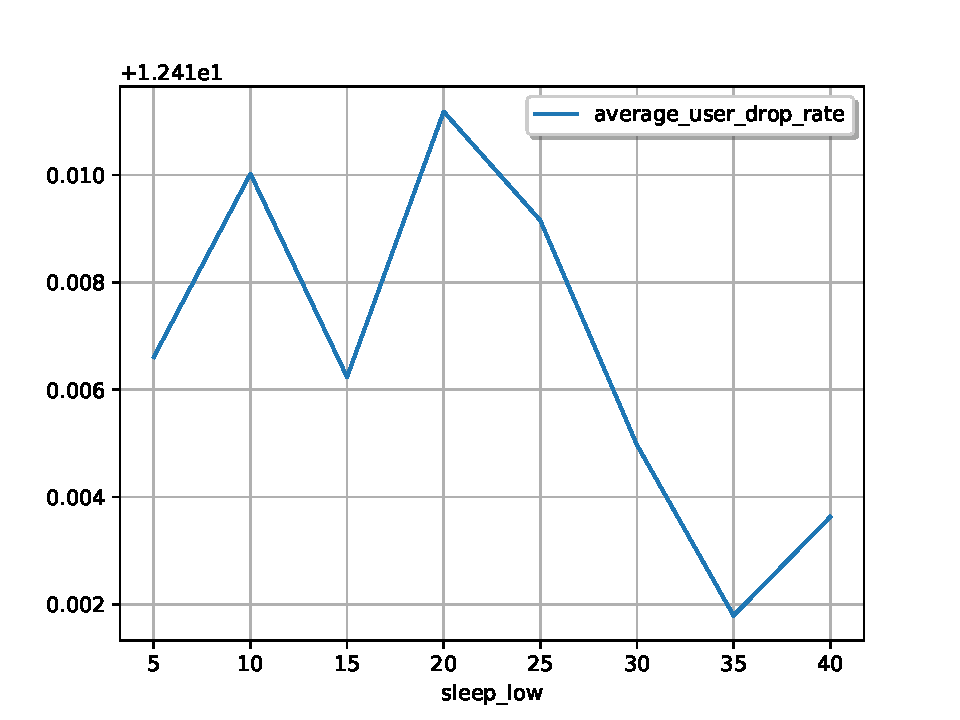
\includegraphics[scale=0.65]{img/drop_rate_lambda_50.pdf} 
\caption{Wykres procentu traconych użytkowników w funkcji wartości parametru L. W trakcie symulacji parametr $\lambda$ wynosił 50.}
\label{dropped_users_iter_l3}
\end{figure}
\begin{figure}[h!]
\center
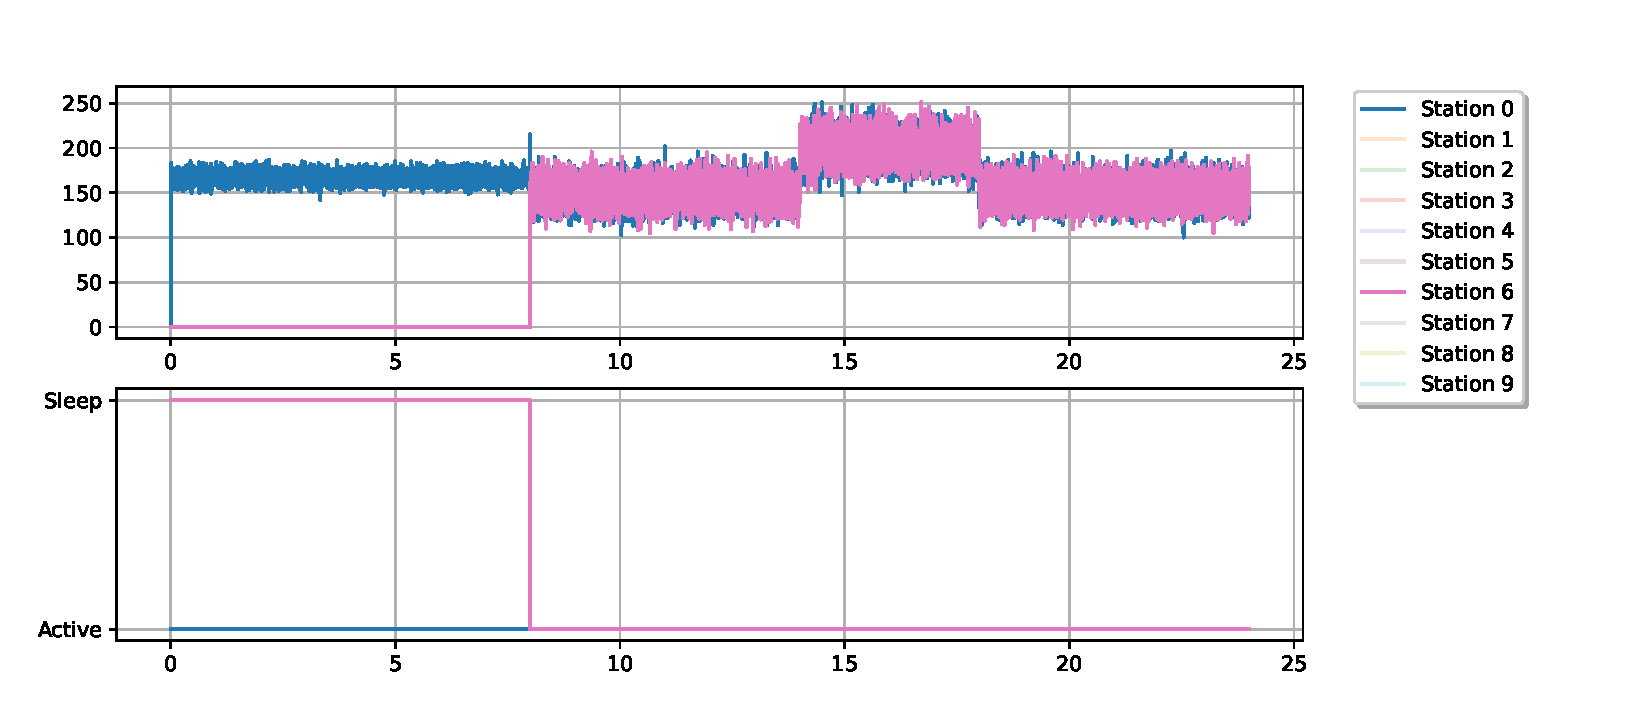
\includegraphics[scale=0.65]{img/usage_over_time.pdf} 
\caption{Wykres zużycia zasobów stacji bazowych nr 0 i 6 w funkcji czasu symulacji}
\label{usage_over_time}
\end{figure}

\newpage
\subsection{Wyznaczenie uśrednionych parametrów systemu} \label{get_params_section}
Uśrednione parametry systemu wyznaczono symulacją uśrednioną z 20 iteracji, gdzie parametr $\lambda$ wynosił 43 a próg L był równy 20\%. Wyniki symulacji przedstawiono na rysunku \ref{sim_results_average} oraz w tabeli \ref{params_table}. Ponieważ ilość użytkowników napływających do systemu była większa od pojemności stacji bazowych, wszystkie uśpione stacje zostały wybudzone w początkowej fazie symulacji, stąd średnia moc pobierana przez stacje wynosi 200W a średni czas uśpienia to 0\%. 
\newline\newline
\begin{table}[h]
\caption{Wartość wyznaczonych parametrów}
\label{params_table}
\begin{center}
	\renewcommand{\arraystretch}{1.5}
	\begin{tabular}{|l|l|}
	\hline 
	Średnie dobowe zużycie energii & 199.99W \\ 
	\hline 
	Średnia dobowa zajętość bloków zasobów & 84.88\% \\ 
	\hline 
	Średnia dobowa liczba traconych zgłoszeń & 4.89\% \\ 
	\hline 
	Średni czas uśpienia stacji bazowej & 0\% \\ 
	\hline 
	\end{tabular} 
\end{center}
\end{table}

\begin{figure}[h]
\center
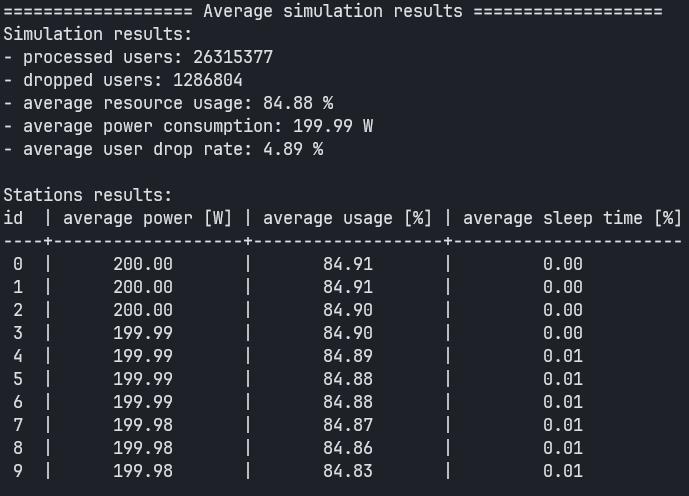
\includegraphics[scale=0.6]{img/sim_results_sleep_lambda_43.png} 
\caption{Raport wynikowy symulacji dla parametrów $\lambda$ = 43 oraz L = 20, uśredniony z 20 iteracji}
\label{sim_results_average}
\end{figure}

\subsection{Wyznaczenie średniego zużycia energii w funkcji progu L} \label{power_l_plot}
Symulację wykonano dla wartości progu L z zakresu $<5:40>$ z krokiem równym 5, dla wartości parametru $\lambda$ = 20. Każda próbka wykresu, przedstawionego na rysunku \ref{power_usage_lambda_sleep}, została uśredniona z 20 iteracji. Z analizy uzyskanego wykresu wynika że wraz ze wzrostem progu uśpienia L, dla niskich wartości $\lambda$, średni pobór mocy przez stacje bazowe maleje. Na rysunku \ref{usage_over_time_sleep} przedstawiono wykres zużycia zasobów stacji 0 i 7 w funkcji czasu. Stacja numer 7 została aktywowany po rozpoczęciu fazy największego ruchu (gdy współczynnik $\lambda$ = 1) oraz została wyłączona gdy generowany ruch zmalał. Dzięki temu średni pobór mocy w systemie zmalał, względem symulacji gdy próg uśpienia miał niższą wartość lub gdy logika odpowiedzialna za usypianie stacji była wyłączona.

\begin{figure}[h!]
\center
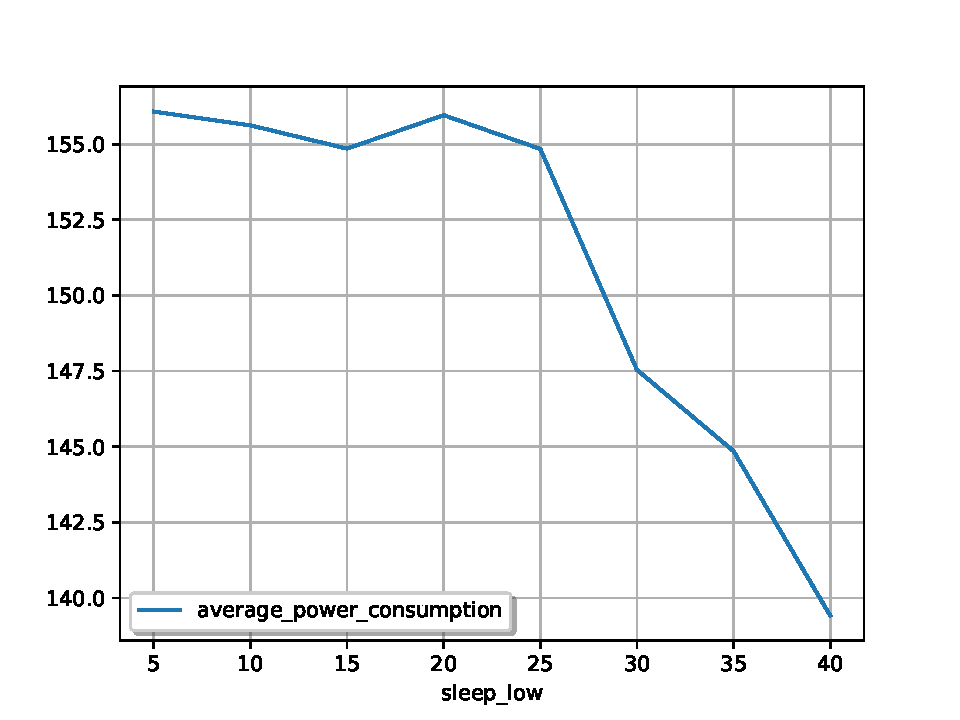
\includegraphics[scale=0.65]{img/power_usage_lambda_20.pdf} 
\caption{Wykres średniego poboru mocy przez stacje bazowe w funkcji wartości progu L. W trakcie symulacji parametr $\lambda$ był równy 20}
\label{power_usage_lambda_sleep}
\end{figure}

\begin{figure}[h]
\center
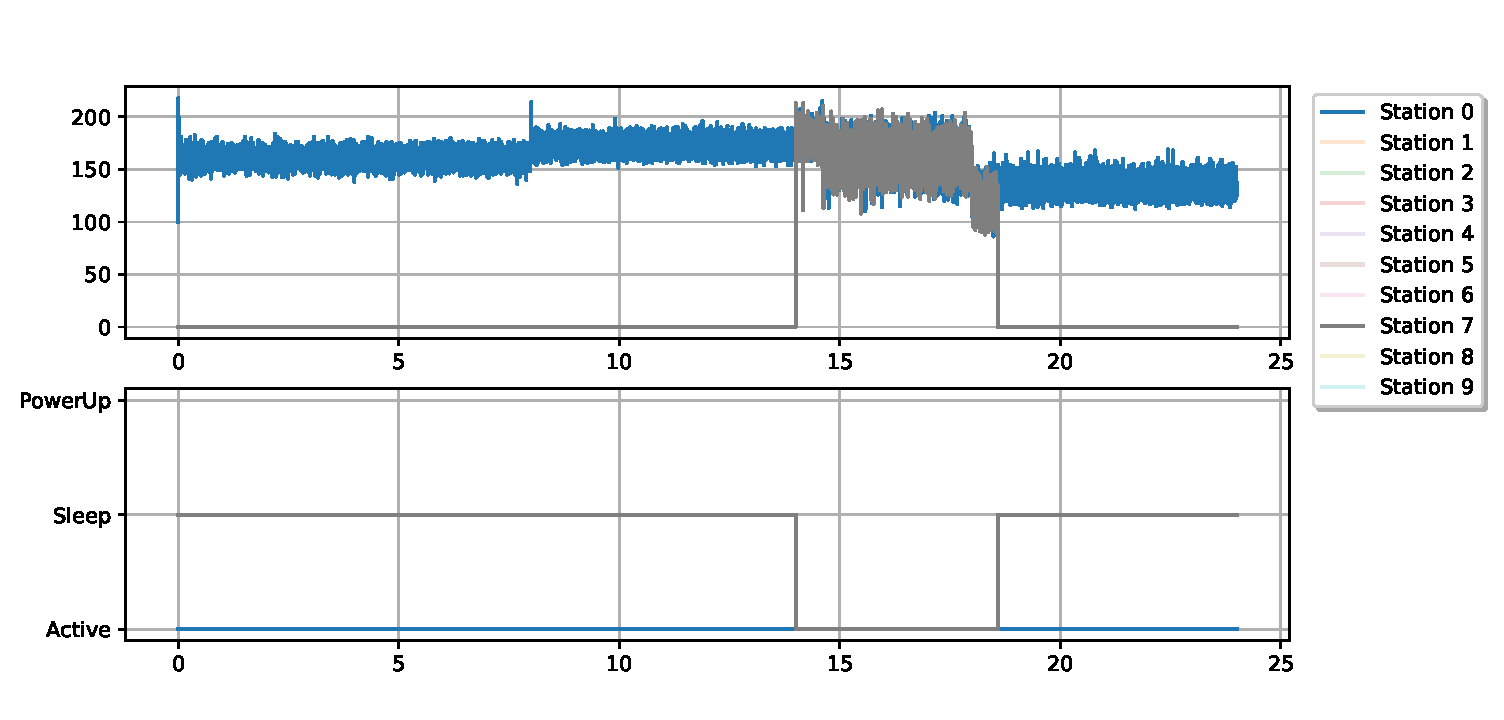
\includegraphics[scale=0.65]{img/usage_over_time_sleep.pdf} 
\caption{Wykres średniego poboru mocy przez stacje bazowe w funkcji wartości progu L}
\label{usage_over_time_sleep}
\end{figure}

\subsection{Wyznaczenie średniej ilości traconych użytkowników w funkcji progu L} \label{drop_l_plot}
Z przyczyn wymienionych w sekcji \ref{drop_rate_5_section}, liczba traconych użytkowników nie zależy od wartości progu L oraz, ponieważ w trakcie symulacji parametr $\lambda$ był równy 20, jest równa zero.

\begin{figure}[h]
\center
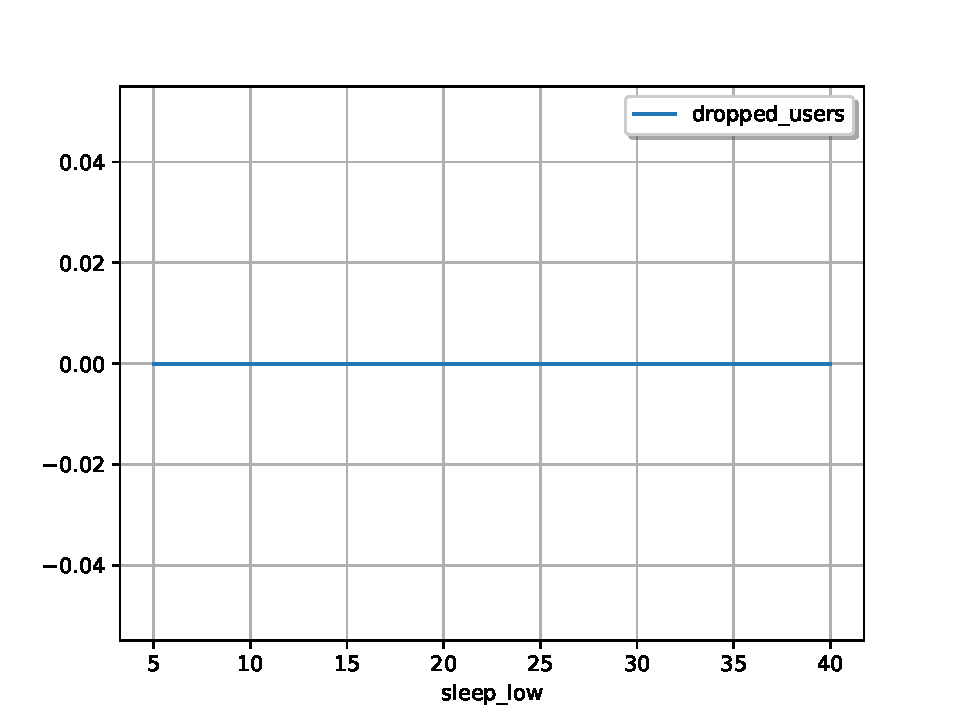
\includegraphics[scale=0.65]{img/dropped_users_lambda_20.pdf} 
\caption{Wykres średniego ilości traconych użytkowników w funkcji wartości progu L}
\label{drop_over_time_sleep}
\end{figure}
